\subsection{Once-through results}

\begin{frame}
    \frametitle{Number of reactors}
    %\begin{columns}
        %\column[t]{4.3cm}
            \begin{itemize}
                \item Number of reactors deployed scales with the power 
                      output of each reactor type
                \item Scenario 2 (MMR) deploys the most reactors
                \item Scenario 3 (Xe-100) deploys the fewest reactors
                \item Similar number of Xe-100s and VOYGRs are deployed
                \item Scenarios 4 (Xe-100+MMR), 6 (Xe-100+VOYGR), and 7 
                      (Xe-100+VOYGR+MMR) mostly deploy Xe-100s 
                \item Scenario 5 (MMR+VOYGR) mostly deploys VOYGRs
            \end{itemize}
        %\column[t]{5.7cm}
        %\vspace{-0.5cm}
        \begin{figure}
        \begin{subfigure}{0.48\textwidth}
                \centering
                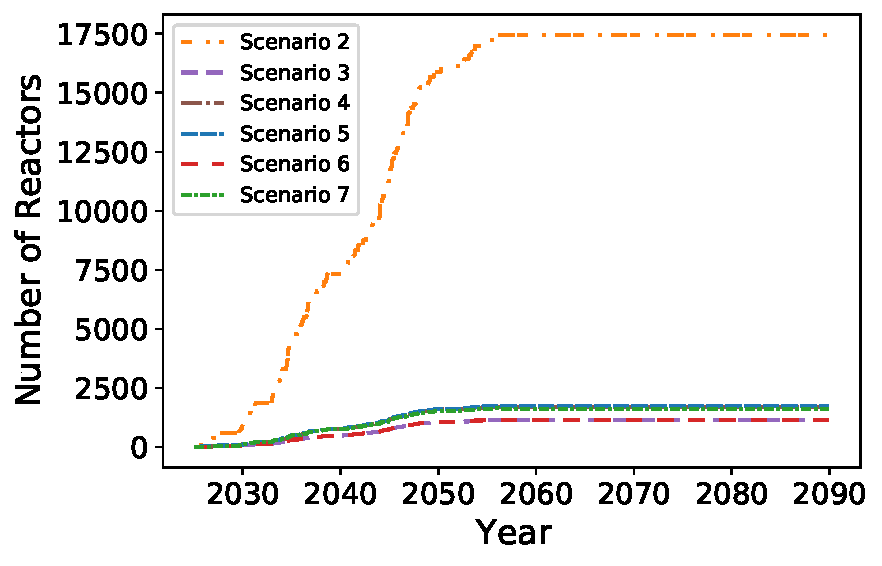
\includegraphics[width=\textwidth]{nogrowth_reactors.pdf}
        \end{subfigure}
        \hfill
        \begin{subfigure}{0.48\textwidth}
            \centering
            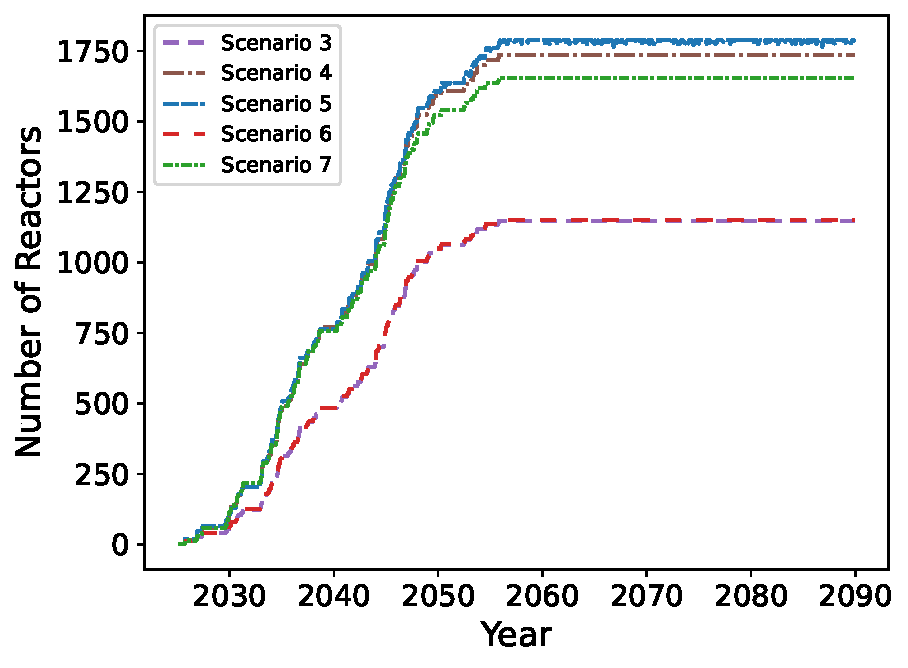
\includegraphics[width=\textwidth]{nogrowth_reactors_3-7.pdf}
        \end{subfigure}
        \vspace{-0.15cm}
        \caption{Number of advanced reactors deployed in Scenarios 2-7 (left)
        and Scenarios 3-7 (right).}
        \end{figure}
    %\end{columns}
\end{frame}

\begin{frame}
    \frametitle{Reactor designs drives the uranium mass required}
    \begin{columns}
        \column[t]{4.5cm}
            \begin{itemize}
                \item Scenario 5 (MMR + VOYGR) requires the largest average mass of 
                      enriched uranium
                \item Scenario 2 (MMR) requires the largest mass of \gls{HALEU}
                \item Scenario 3 (Xe-100) requires the smallest mass of enriched 
                      uranium
                \item Scenario 5 (MMR + VOYGR) requires the smallest mass of \gls{HALEU}
            \end{itemize}
        \column[t]{5.5cm}
        \vspace{-0.8cm}
            \begin{figure}
                \centering
                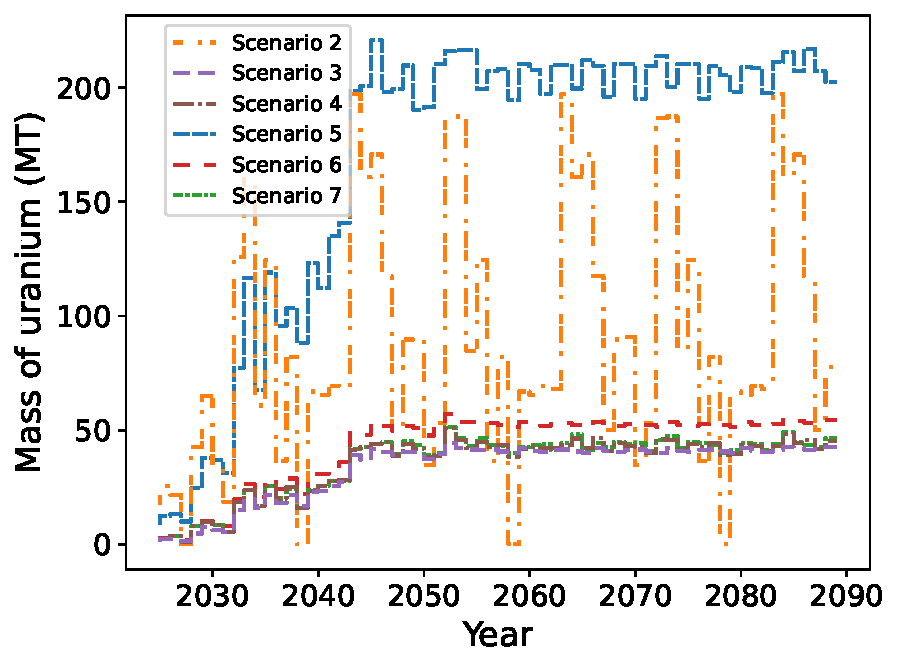
\includegraphics[scale=0.43]{nogrowth_AR_uranium.pdf}
                \caption{Annual average mass of enriched uranium required to fuel
                advanced reactors in Scenarios 2-7.}
                \label{fig:uranium}

        \end{figure}
    \end{columns}
\end{frame}

\begin{frame}
    \frametitle{Advanced reactor designs}
    \begingroup
        \renewcommand{\arraystretch}{1.5}
        \begin{table}
            \small
            \caption{Advanced reactor design specifications}
            \label{tab:reactor_summary}
            \begin{tabular}{ c c c c }
                \hline
                Design Criteria & MMR 
                    \cite{noauthor_usnc_2021} & 
                    Xe-100 \cite{mulder_overview_2021} & 
                    VOYGR \cite{nuscale_chapter_2020-1,reyes_nuscale_2021,reyes_correction_2022}\\\hline
                Power (MWe) & 5 & 80 & 77\\
                Power (MWth) & 15 & 200 & 250\\
                Enrichment (\% $^{235}U$) & 19.75 & 15.5 & 4.09 \\
                Cycle Length (yr) & 20 & Online & 1.5 \\
                Number of cycles & 1 & 6 & 3\\
                Reactor Lifetime (yr) & 20 & 60 & 60\\
                Burnup ($\frac{MWd}{kg U}$) & 82 & 168 & 45\\
                \hline
            \end{tabular}
        \end{table}   
    \endgroup
    \begin{equation*}
        \text{mass (kg)} = \frac{\text{Power (MWth) * cycle length (d)*number of cycles}}{\text{Burnup (MWd/kg)}}
        \label{eq:fuel_mass}
    \end{equation*}
\end{frame}

\begin{frame}
    \frametitle{\gls{SWU} capacity is a function of product mass and assay}
    \begin{columns}
        \column[t]{4.3cm}
            \begin{itemize}
                \item Follows similar pattern to feed uranium  mass 
                \item Scenario 2 (MMR) requires the largest average \gls{SWU} 
                \item The other scenarios are comparable for the average 
                      capacity they require
                \item \gls{SWU} capacity is a function of product mass and 
                      product assay
                
            \end{itemize}
        \column[t]{5.7cm}
        \vspace{-1cm}
        \begin{figure}
                \centering
                \includegraphics[scale=0.43]{nogrowth_AR_swu.pdf}
                \caption{Annual average \gls{SWU} capacity required to produce 
                enriched uranium for and advanced reactors in Scenarios 2-7.}
                \label{fig:swu}
        \end{figure}
    \end{columns}
\end{frame}

\begin{frame}
    \frametitle{\gls{SNF} discharged follows with fuel mass}
    \begin{columns}
        \column[t]{4.3cm}
            \begin{itemize}
                \item Scenario 5 (MMR + VOYGR) discharges the largest mass of \gls{SNF}
                \item Scenario 3 (Xe-100) discharges the least \gls{SNF}
                \item Scenario 2 (MMR) discharges \gls{SNF} the latest
                \item Cumulative masses range between 25,654 MT (Scenario 3) to 
                      112,913 MT (Scenario 5)
                
            \end{itemize}
        \column[t]{5.7cm}
        \vspace{-1cm}
        \begin{figure}
                \centering
                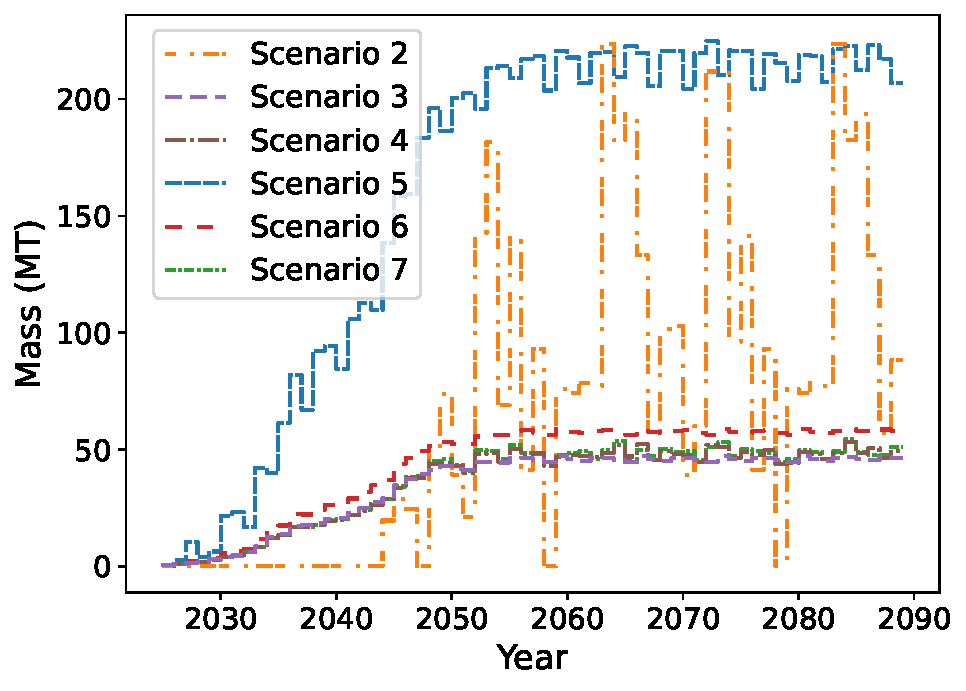
\includegraphics[scale=0.43]{nogrowth_AR_waste.pdf}
                \caption{Annual average mass of \gls{SNF} discharged from 
                advanced reactors in Scenarios 2-7.}
                \label{fig:waste}
        \end{figure}
    \end{columns}
\end{frame}